\documentclass[table]{beamer}
\usepackage[utf8]{inputenc}
\usepackage[brazilian]{babel}
\usepackage{amsmath}
\usepackage{graphicx}
\usepackage{hyperref}
\usepackage{ragged2e}   
\usepackage{epstopdf}
\usepackage{multirow}
\usepackage{minted}
\usepackage{booktabs}

\setbeamertemplate{sidebar right}{}
\setbeamertemplate{footline}{%
\hfill\usebeamertemplate***{navigation symbols}
\hspace{1cm}\insertframenumber{}/\inserttotalframenumber}

\addtobeamertemplate{block begin}{}{\justifying}  %new code

\setbeamertemplate{footline}
{
  \leavevmode%
  \hbox{%
  \begin{beamercolorbox}[wd=.333333\paperwidth,ht=2.25ex,dp=1ex,center]{author in head/foot}%
    \usebeamerfont{author in head/foot}\insertsection
  \end{beamercolorbox}%
  \begin{beamercolorbox}[wd=.333333\paperwidth,ht=2.25ex,dp=1ex,center]{title in head/foot}%
    \usebeamerfont{title in head/foot}\insertsubsection
  \end{beamercolorbox}%
  \begin{beamercolorbox}[wd=.333333\paperwidth,ht=2.25ex,dp=1ex,right]{date in head/foot}%
    \usebeamerfont{date in head/foot}\insertshortdate{}\hspace*{2em}
    \insertframenumber{} / \inserttotalframenumber\hspace*{2ex} 
  \end{beamercolorbox}}%
  \vskip0pt%
}

\begin{document}

\begin{frame}
   \frametitle{Compiladores}
   \large
   \begin{center}
   Análise Sintática Ascendente
   \end{center}
   \scriptsize
   \begin{center}
      João Marcelo Uchôa de Alencar \\
      joao.marcelo@ufc.br \\
      UFC-Quixadá
   \end{center}
\end{frame}

\begin{frame}
   \frametitle{Introdução}
   \begin{itemize}
      \item \textbf{Análise Sintática LR(1)}: entrada processada da esquerda para a direita, mas a derivação produzida é uma derivação à direita, analisando um símbolo da entrada;
      \item \textbf{Análise Sintática LR(0)}: não analisa o símbolo na entrada, apenas quando ele já aparece na pilha;
      \item \textbf{Análise Sintática SLR(1)}: versão melhorada da LR(0), com verificação da entrada;
      \item \textbf{Análise Sintática LALR(1)}: mais poderoso que a SLR(1).
   \end{itemize}
   \begin{center}
   Ordem de complexidade e poder de expressão: \\
   $LR(0) < SLR(1) < LALR(1) < LR(1)$
   \end{center}
   \textbf{Recursão à esquerda} não é um problema para a análise ascendente. Por que?
\end{frame}

\begin{frame}
   \tableofcontents
\end{frame}

\section{Visão Geral}
\begin{frame}[fragile]
   \frametitle{Visão Geral}
   A \textbf{pilha} conterá tanto marcas como não terminais, e também informações adicionais de estados.
   \begin{minted}{text}
$      ...        CadeiaEntrada $
       ...             ...      $
       ...             ...      $
$ SímboloInicial                $ aceita    
   \end{minted}
   Duas operações possíveis:
   \begin{enumerate}
      \item \textbf{Carrega} (\textit{shift}) um terminal do topo da entrada para o topo da pilha;
      \item \textbf{Reduz} (\textit{reduce})  uma cadeia $\alpha$ do topo da pilha para um não terminal A, dada a escolha BNF $A\to\alpha$.
   \end{enumerate}
   As gramáticas são aumentadas com um novo \textbf{símbolo inicial}, com uma única produção unitária para o símbolo inicial anterior.
\end{frame}

\begin{frame}
   \frametitle{Visão Geral - Exemplo}
   $S^{'}\to S$ \\
   $S\to(S)S|\varepsilon$ \\
   \\
   Considerando a cadeia $()$ temos:

   \begin{table}
      \begin{tabular}{|c|l|r|l|}
      \hline
      & Pilha de Análise Sintática & Entrada & Ação \\
      \hline 
      1 & \$        & ()\$ & carrega                         \\
      2 & \$(       &  )\$ & reduz $S\to\varepsilon$         \\
      3 & \$(S      &  )\$ & carrega                         \\
      4 & \$(S)     &   \$ & reduz $S\to\varepsilon$         \\
      5 & \$(S)S    &   \$ & reduz $S\to(S)S$                \\
      6 & \$S       &   \$ & reduz $S^{'}\to S$              \\
      7 & \$$S^{'}$ &   \$ & aceita                          \\
      \hline
      \end{tabular}
   \end{table}
\end{frame}

\begin{frame}
   \frametitle{Visão Geral - Exemplo}
   $E^{'}\to E$ \\
   $E\to E+n|n$ \\
   \\
   Considerando a cadeia $n+n$ temos:

   \begin{table}
      \begin{tabular}{|c|l|r|l|}
      \hline
      & Pilha de Análise Sintática & Entrada & Ação \\
      \hline 
      1 & \$        & n+n\$ & carrega                         \\
      2 & \$n       &  +n\$ & reduz $E\to n$         \\
      3 & \$E       &  +n\$ & carrega                         \\
      4 & \$E+      &   n\$ & carrega   \\
      5 & \$E+n     &    \$ & reduz $E\to E + n$                \\
      6 & \$E       &    \$ & reduz $E^{'}\to E$              \\
      7 & \$$E^{'}$ &    \$ & aceita                          \\
      \hline
      \end{tabular}
   \end{table}
\end{frame}

\begin{frame}
   \frametitle{Visão Geral}
   \begin{itemize}
      \item Um analisador ascendente pode carregar os símbolos de entrada para a pilha até determinar que ação deve executar;
      \item ao mesmo tempo, ele pode precisar de outros elementos da pilha, além do topo, para determinar a ação a ser executada;
      \item \textbf{verificações à frente na pilha}: autômato finito determinístico de \textit{itens};
      \item as verificações na pilha não eliminam a necessidade de analisar a entrada;
      \item a forma em que a verificação é feita é o que difencia o poder e a complexidade dos algoritmos ascendentes.
   \end{itemize}
\end{frame}

\begin{frame}
   \frametitle{Visão Geral - Conceitos}
   Um analisador \textit{shift-reduce} acompanha uma derivação à direita da cadeia, mas os passos ocorrem em ordem inversa:
   \begin{itemize}
      \item \textbf{Forma sentencial à direita}: é uma cadeia intermediária e terminais e não terminais na derivação;
      \item \textbf{prefixo viável}: porção da forma sentencial à direita que está na pilha em um dado momento da derivação;
      \item \textbf{gancho}: cadeia de símbolos no topo da pilha que casa com o lado direito de uma produção $+$ posição na forma sentencial à direita onde ocorre $+$ produção para a redução.
   \end{itemize}
   A tarefa principal de um analisador carrega-reduz é determinar o gancho seguinte em uma análise sintática.
\end{frame}

\section{Análise Sintática LR(0)}
\begin{frame}
   \frametitle{Análise Sintática LR(0)}
   \begin{itemize}
      \item Um \textbf{item LR(0)} de uma gramática livre de contexto é uma escolha de produção com uma posição identificada em seu lado direito; 
      \item se $A\to\alpha$ e $\beta\gamma=\alpha$, $A\to\beta.\gamma$ é um item LR(0). 
   \end{itemize}  
   Para os exemplos: \\
   \begin{columns}
   \begin{column}{0.4\textwidth}
   $S^{'}\to.S$  \\ 
   $S^{'}\to S.$ \\
   $S\to.(S)S$   \\
   $S\to(.S)S$   \\
   $S\to(S.)S$   \\
   $S\to(S).S$   \\
   $S\to(S)S.$   \\
   $S\to.$   \\
   \end{column}
   \begin{column}{0.4\textwidth}
   $E^{'}\to.E$   \\
   $E^{'}\to E.$  \\
   $E\to.E + n$   \\
   $E\to E. + n$  \\
   $E\to E +. n$  \\
   $E\to E + n.$  \\
   $E\to .n$      \\
   $E\to n.$      \\
   \end{column}
   \end{columns}
   \vspace{0.3cm}
   Um item registra um passo intermediário no reconhecimento do lado direito de uma escolha.
\end{frame}

\begin{frame}
   \frametitle{Autômatos Finitos para Itens}
   \begin{block}{Controlar as Opções de Redução}
   Os itens LR(0) podem ser utilizados como os estados de um autômato finito que mantém as informações sobre a pilha de análise sintática e o \textbf{progresso} de uma análise \textit{shift-reduce}.
   \end{block}
   Etapas:
   \begin{enumerate}
      \item Construção de um NFA a partir dos itens;
      \item utilizar a construção de subconjuntos para definir um DFA.
   \end{enumerate}
\end{frame}

\begin{frame}
   \frametitle{Construção de um NFA dos Itens}
    Considere $A\to\alpha\gamma$ e $\gamma$ inicia com $X$ (terminal ou não), tal que $A\to\alpha.X\eta$. Então existe a transição para o item $A\to\alpha X.\eta$: 
   \begin{center}
   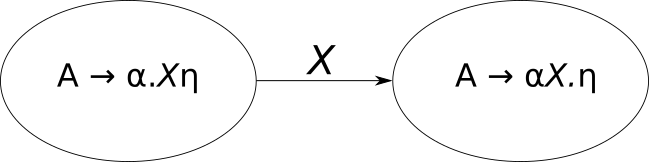
\includegraphics[scale=0.4]{figuras/nfa1.png}
   \end{center}
   Se $X$ for marca, carregar $X$ da entrada para o topo da pilha. Se X for não terminal, ele só pode aparecer por redução. Logo, para $X\to\beta$, $\beta$ deve ser reconhecido \textit{simultaneamente} com a transição acima.
   \begin{center}
   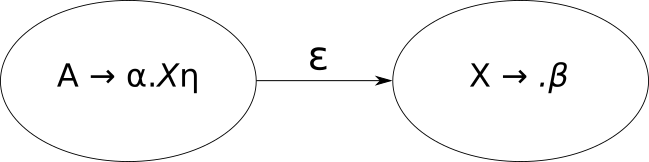
\includegraphics[scale=0.4]{figuras/nfa2.png}
   \end{center}
   Para todas as possibilidades de $\beta$, $X\to\beta$.
\end{frame}

\begin{frame}
   \frametitle{Exemplos}
   Vamos construir os NFAs para os exemplos abaixo. \\
   \begin{columns}
   \begin{column}{0.4\textwidth}
   $S^{'}\to.S$  \\ 
   $S^{'}\to S.$ \\
   $S\to.(S)S$   \\
   $S\to(.S)S$   \\
   $S\to(S.)S$   \\
   $S\to(S).S$   \\
   $S\to(S)S.$   \\
   $S\to.$   \\
   \end{column}
   \begin{column}{0.4\textwidth}
   $E^{'}\to.E$   \\
   $E^{'}\to E.$  \\
   $E\to.E + n$   \\
   $E\to E. + n$  \\
   $E\to E +. n$  \\
   $E\to E + n.$  \\
   $E\to .n$      \\
   $E\to n.$      \\
   \end{column}
   \end{columns}
   \vspace{1.0cm}
   Depois, usar a \textbf{construção de subconjuntos} para transformá-los em DFAs.
\end{frame}

\begin{frame}
   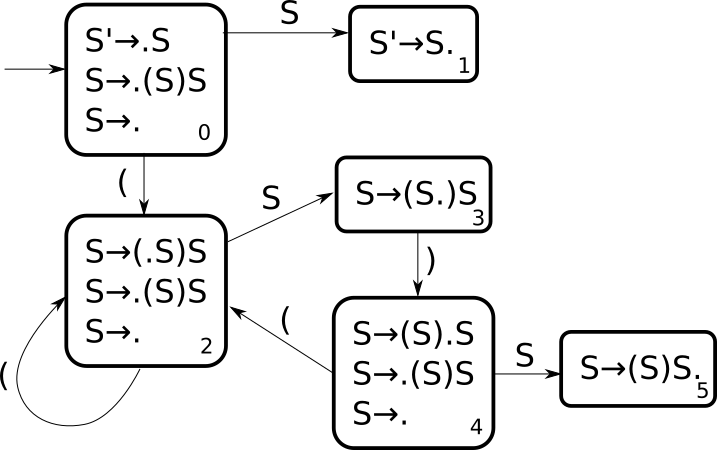
\includegraphics[width=\linewidth,height=\textheight,keepaspectratio]{figuras/ssadfa.png}
\end{frame}

\begin{frame}
   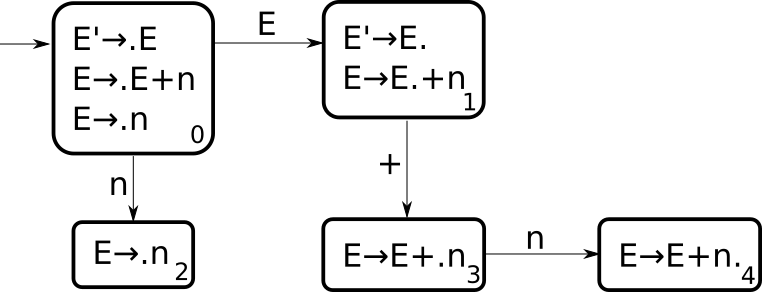
\includegraphics[width=\linewidth,height=\textheight,keepaspectratio]{figuras/endfa.png}
\end{frame}

\begin{frame}
   \frametitle{Definições Adicionais sobre os Autômatos LR(0)}
   \begin{itemize}
      \item \textbf{Itens de fecho}: itens que são adicionados a um estado durante um $\varepsilon$-fecho;
      \item \textbf{itens de núcleo}: itens que geram estados alvos de transições que não são $\varepsilon$-transições.
   \end{itemize}
   Os itens de núcleo determinam de forma única o estado e suas transições.
\end{frame}

\begin{frame}
   \frametitle{O Algoritmo de Análise Sintática LR(0)}
   A pilha passa a conter não apenas símbolos, mas também número de estados. Início:
   \begin{table}
   \begin{tabular}{|l|l|}
   \hline
   Pilha de Análise Sintática & Entrada \\
   \hline 
   \$ 0                       & \textit{CadeiaEntrada} \$ \\
   \hline
   \end{tabular}
   \end{table}
   Carregar a marca $n$ para a pilha e ir para o estado 2:
   \begin{table}
   \begin{tabular}{|l|l|}
   \hline
   Pilha de Análise Sintática & Entrada \\
   \hline 
   \$ 0$n$2                    & \textit{Restante da CadeiaEntrada} \$ \\
   \hline
   \end{tabular}
   \end{table}
   O algoritmo escolhe uma ação com base no estado corrente do DFA, que está no topo da pilha.
\end{frame}

\begin{frame}
   \frametitle{O Algoritmo de Análise Sintática LR(0)}
   Seja $s$ o estado corrente (topo da pilha), ações:
   \begin{enumerate}
      \item Se o estado $s$ contiver um item da forma $A\to\alpha.X\beta$, $X$ terminal, então a \textbf{ação} é carregar a marca da entrada para a pilha. Se a marca for $X$ e $s$ contiver o item $A\to\alpha.X\beta$, então o novo estado a ser empilhado é o que contiver $A\to\alpha X.\beta$. Caso contrário, erro.
      \item Se o estado $s$ contiver um item completo $A\to\gamma.$ então a \textbf{ação} é reduzir por $A\to\gamma$. Uma redução por $S^{'}\to S$ equivale a aceitação, se a entrada estiver vazia. Caso contrário:
      \begin{itemize}
         \item Remover $\gamma$ e os estados correspondentes;
	 \item retorne o DFA para o estado no qual iniciou a construção de $\gamma$;
	 \item o estado atual deve conter item da forma $B\to\alpha.A\beta$;
	 \item coloque $A$ na pilha e atualize o estado para o que contiver $B\to\alpha A.\beta$.
      \end{itemize}
   \end{enumerate}
\end{frame}

\begin{frame}
   \frametitle{Conflitos da Análise Sintática LR(O)}
   Uma gramática é dita LR(0) se as regras anteriores não forem ambíguas. Tipos de conflitoss:
   \begin{itemize}
      \item \textbf{Conflito carrega-reduz}: um estado contém tanto um item $A\to\alpha.$ quanto $A\to\alpha.X\beta$;
      \item \textbf{conflito reduz-reduz}:  um estado contém tanto um item $A\to\alpha.$ quanto $B\to\beta.$;
  \end{itemize}
  Nenhuma das gramáticas apresentadas como exemplo até agora são LR(0). Por quê?
\end{frame}

\begin{frame}
   \frametitle{Exemplo de Gramática LR(0)}
   Para a gramática: \\
   $A\to(A)|a$ \\
   Temos o seguinte autômatos de itens: \\
   \begin{center}
   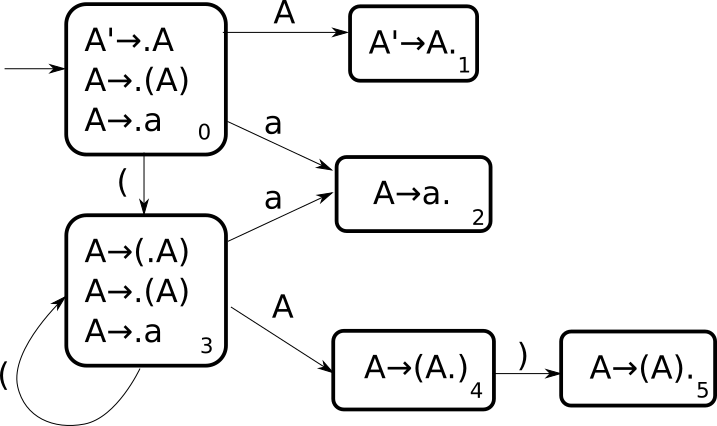
\includegraphics[scale=0.4]{figuras/aadfa.png}
   \end{center}
   Vamos fazer o reconhecimento de ((a))?
\end{frame}

\section{Análise Sintática SLR(1)}
\begin{frame}
   \frametitle{Análise Sintática SLR(1)}
   Vamos aumentar o poder da análise LR(0):
   \begin{enumerate}
      \item Consultar a marca de entrada \textit{antes} de carregar, para garantir que exista uma transição apropriada no DFA;
      \item utilizar o conjunto Sequência de um não-terminal para decidir se uma redução deve ser efetuada.
   \end{enumerate}
\end{frame}

\begin{frame}
   \frametitle{Algoritmo de Análise Sintática SLR(1)}
   Seja $s$ o estado corrente (topo da pilha), ações:
   \begin{enumerate}
      \item Se o estado $s$ contiver um item da forma $A\to\alpha.X\beta$, $X$ terminal, \textbf{e X for a marca seguinte na cadeia de entrada}, então a \textbf{ação} é carregar a marca da entrada para a pilha. O novo estado a ser empilhado é o que contiver $A\to\alpha X.\beta$.
      \item Se o estado $s$ contiver um item completo $A\to\gamma.$, \textbf{e a marca seguinte na cadeia de entrada estiver em Sequência(A)}, então a \textbf{ação} é reduzir por $A\to\gamma$. Uma redução por $S^{'}\to S$ equivale a aceitação, se a entrada for \$. Caso contrário:
      \begin{itemize}
         \item Remover $\gamma$ e os estados correspondentes;
	 \item retorne o DFA para o estado no qual iniciou a construção de $\gamma$;
	 \item o estado atual deve conter item da forma $B\to\alpha.A\beta$;
	 \item coloque $A$ na pilha e atualize o estado para o que contiver $B\to\alpha A.\beta$.
      \end{itemize}
      \item Se a marca de entrada for tal que nenhum caso acima se aplique, erro!
   \end{enumerate}
\end{frame}

\begin{frame}
   \frametitle{Conflitos da Análise Sintática SLR(1)}
   Dizemos que uma gramática é SLR(1) se a aplicação das regras não resultarem em ambiguidade. As duas condições devem ser satisfeitas:
   \begin{enumerate}
      \item Para qualquer item $A\to\alpha.X\beta$ em $s$ em que $X$ for um não terminal, não existe um item completo $B\to\gamma.$ em $s$ com X em Sequência(B);
      \item Para quaisquer dois itens completos $A\to\alpha.$ e $B\to\beta.$ em $s$, Sequência(A) $\cap$ Sequência(B) é vazio.
   \end{enumerate}
   A violação da primeira condição representa um \textbf{conflito carrega-reduz}. A violação da segunda condição representa um \textbf{conflito reduz-reduz}.
\end{frame}

\begin{frame}
   \frametitle{Construção da Tabela SLR(1)}
   Percorrendo o autômato gerado, considerando cada terminal e não-terminal, podemos construir a tabela SLR(1). Dada a gramática \\
   $E^{'}\to E$ \\
   $E\to E+n|n$ \\
   e o autômato gerado para ela e o fato de que Sequência(E)$=\{\$\}$ e Sequência(E')$=\{\$,+\}$, temos a tabela:
   \begin{table}
   \begin{tabular}{|c|c|c|c|c|}
   \hline
   \textbf{Estado} & \multicolumn{3}{c|}{\textbf{Entrada}} & \textbf{Ir-para}\\
   \hline 
   & $n$ & $+$ & \$ & $E$  \\
   \hline
   0 & s2 &               &               & 1 \\
   1 &    & s3            & aceita        & \\
   2 &    & r($E\to n$)   & r($E\to n$)   & \\
   3 & s4 &               &               & \\
   4 &    & r($E\to E+n$) & r($E\to E+n$) & \\
   \hline
   \end{tabular}
   \end{table}
   Vamos fazer a análise da cadeia $n+n+n$.
\end{frame}

\begin{frame}
   \frametitle{Regras para Eliminar Ambiguidades}
   No caso da SLR(1), podemos tomar algumas atitudes para eliminar ambiguidades:
   \begin{itemize}
      \item No caso dos conflitos carrega-reduz, existe uma regra natural, que é sempre preferir carregar em vez de reduzir;
      \item o caso dos conflitos reduz-reduz, não há solução geral, geralmente é indício de erro no projeto.
   \end{itemize}
   A solução de carregar no lugar de reduzir tem algum impacto no problema do \textit{else} aninhado?
\end{frame}

\begin{frame}
   \frametitle{Exemplo de Eliminação de Ambiguidade}
   Considere a gramática: \\
   \\
   $\textit{declaração}\to \textit{if-stmt}|\textbf{outra}$ \\
   $\textit{if-decl} \to \textbf{if}(exp) \textit{declaração}$ \\
   $|\textbf{if}(exp)\textit{declaração }\textbf{else }\textit{declaração}$ \\
   $exp\to\textbf{0}|\textbf{1}$ \\
   \\
   É notoriamente ambígua. Vamos simplificá-la para poder criar o autômato: \\
   \\
   $S\to I|\textbf{outra}$ \\
   $\textbf{I}\to\textbf{if }S|\textbf{if }S\textbf{ else }S$ \\
   \\
   Temos a seguinte propriedade: \\
   Sequência($S$) = Sequência($I$) = $\{\$, else\}$
\end{frame}

\begin{frame}
   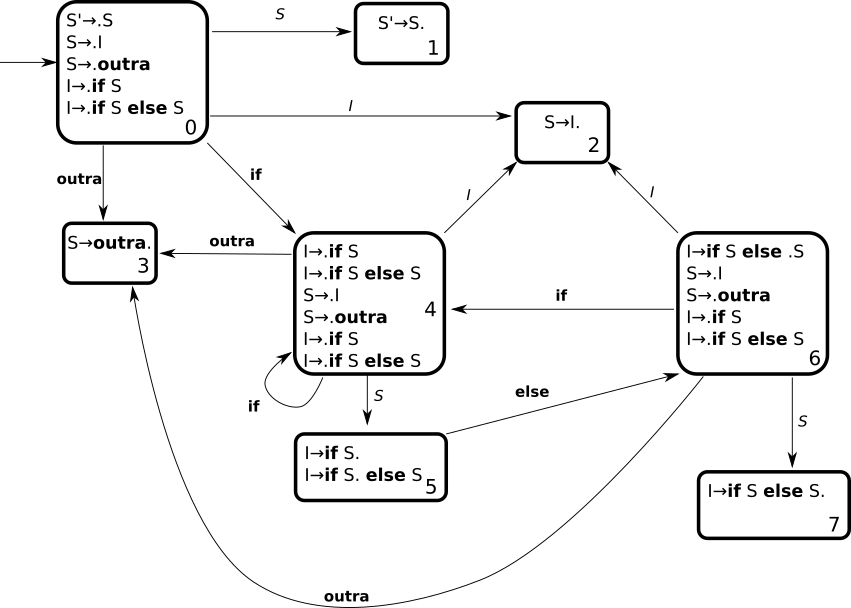
\includegraphics[width=\linewidth,height=\textheight,keepaspectratio]{figuras/ifthenelsedfa.png}
\end{frame}

\begin{frame}
   \frametitle{Exemplo de Eliminação de Ambiguidade}
   O estado 5 tem $\{I\to\textbf{if }S.\text{;}I\to\textbf{if }S.\textbf{ else }S\}$.
   \begin{itemize}
      \item Devemos reduzir nas entradas \textbf{else} e \$ na primeira derivação?
      \item ou devemos  apenas carregar o \textbf{else} na segunda derivação?
   \end{itemize}
   \begin{table}
      \begin{tabular}{|c|c|c|c|c|c|c|}
      \hline
      \textbf{Estado} & \multicolumn{4}{c|}{\textbf{Entrada}} & \multicolumn{2}{c|}{\textbf{Ir-para}} \\
      \hline 
       & if & else & outra & \$ & S & I \\
       \hline
       0 & s4 &    & s3 &        & 1 & 2 \\
       1 &    &    &    & aceita &   &   \\
       2 &    & r1 &    & r1     &   &   \\
       3 &    & r3 &    & r2     &   &   \\
       4 & s4 &    & s3 &        & 5 & 2 \\
       5 &    & \textbf{s6} &    & r3     &   &   \\
       6 & s4 &    & s3 &        & 7 & 2 \\
       7 &    & r4 &    & r4     &   &   \\
      \hline
      \end{tabular}
   \end{table}
\end{frame}

\begin{frame}
   \frametitle{Limitações da Análise SLR(1)}
   \begin{columns}
   \begin{column}{0.5\textwidth}
   \small
   $decl\to \textit{ativação-decl}|\textit{atribuição-decl}$ \\
   $\textit{ativação-decl}\to \textbf{identificador}$ \\
   $\textit{atribuição-decl}\to var:=exp$ \\
   $var \to var[exp] | \textbf{identificador}$ \\
   $exp \to var | \textbf{número}$ \\
   \vspace{1.0cm}
   Tanto as atribuições quanto declarações começam com \textbf{identificador}.
   \end{column}
   \begin{column}{0.5\textwidth}
   \small
   Versão simplificada: \\
   $S \to \textbf{id}|V:=E$ \\
   $V \to \textbf{id}$ \\
   $E \to V|\textbf{n}$ \\
   Considere o estado inicial com os itens: \\
   $S^{'} \to .S$ \\
   $S \to .\textbf{id}$ \\
   $S \to .V := E $ \\
   $V \to .\textbf{id}$ \\
   \vspace{1.0cm}
   Há conflito para os terminais \textbf{id}.
   \end{column}
   \end{columns}
   \begin{block}{Algoritmos SLR(k)}
   Considerar algoritmos SLR(k) aumenta a expressividade para esses casos, mas a \textbf{complexidade} se torna intratável.
   \end{block}
\end{frame}

\section{Análise Sintática Geral LR(1) e LALR(1)}
\begin{frame}
   \frametitle{Análise Sintática Geral LR(1) e LALR(1)}
   \begin{itemize}
      \item Podemos resolver o problema anterior com a análise LR(1) \textbf{canônica};
      \item essa análise torna o processo complexo devido ao tamanho do autômato gerado;
      \item uma modificação, LALR(1), permite condensar alguns estados em um autômato menor;
      \item entretanto, para compreender a LALR(1), precisamos entender a LR(1) antes.
   \end{itemize}
\end{frame}

\begin{frame}
   \frametitle{Autômatos Finitos de Itens LR(1)}
   O poder do método LR(1) geral é ele utilizar um DFA novo com as verificações à frente construídas em sua concepção.
   \begin{itemize}
      \item \textbf{Item LR(1)}: par composto por um item LR(0) e uma marca de \textit{verificação à frente};
      \item $[A\to\alpha.\beta, a]$, onde $A\to\alpha.\beta$ é um item LR(0) e $a$ é uma marca. Não é a marca à frente na entrada, mas sim uma informação sobre o que se espera na entrada após uma redução.
   \end{itemize}
   A maior diferença entre os autômatos LR(0) e LR(1) aparece na definição das $\varepsilon$-transições.
\end{frame}

\begin{frame}
   \frametitle{Transições dos Autômatos LR(1)}
   \begin{block}{Transições Determinísticas}
   Dado um item LR(1) $[A\to\alpha.X\gamma,a]$, onde $X$ é qualquer símbolo (terminal ou não), existe uma transição em X para o item LR(1) $[A\to\alpha X.\gamma, a]$. \textbf{Não há mudança no símbolo de verificação}.
   \end{block}

   \begin{block}{Transições $\varepsilon$}
   Dado um item LR(1) $[A\to\alpha.B\gamma,a]$, onde \textbf{B é um não terminal}, existem $\varepsilon$-transições $[B\to.\beta, b]$ para cada produção $B \to \beta$ e cada \textbf{marca} $b$ pertencente a Primeiro($\gamma$a).
   \begin{itemize}
      \item $[A\to\alpha.B\gamma,a]$ indica que reconhecemos B se após ocorrer uma cadeia \textit{derivável} de $\gamma a$, começando por marcas presentes em Primeiro($\gamma a$);
      \item restringimos as capturas à conjuntos $Primeiro$, não $Sequencia$;
      \item a verificação original $a$ só é propagada se $\gamma \Rightarrow \varepsilon$.
   \end{itemize}
   \end{block}
\end{frame}

\begin{frame}
   \frametitle{Exemplo de Autômato LR(1)}
   Considere a gramática: \\
   $A\to(A)|a$ \\
   Vamos construir o autômato LR(1)?
\end{frame}

\begin{frame}
   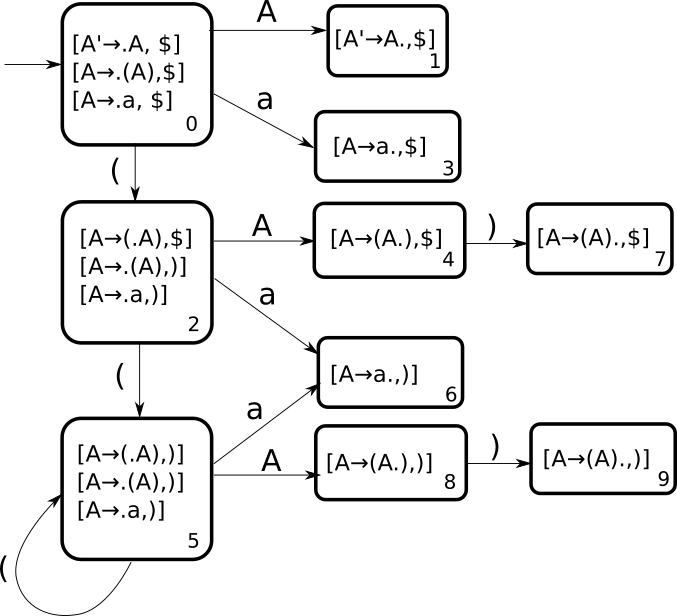
\includegraphics[width=\linewidth,height=\textheight,keepaspectratio]{figuras/aadfalr1.png}
\end{frame}

\begin{frame}
   \frametitle{Tabela LR(1)}
   Enumeramos as produções da gramática:
   \begin{enumerate}
      \item $A\to(A)$
      \item $A\to a$
   \end{enumerate}
   \begin{table}
      \begin{tabular}{|c|c|c|c|c|c|}
      \hline
      \textbf{Estado} & \multicolumn{4}{c|}{\textbf{Entrada}} & \textbf{Ir-para} \\
      \hline 
         & (  & a  & )  & \$     & A  \\
       \hline
       0 & s2 & s3 &    &        & 1  \\
       1 &    &    &    & aceita &    \\
       2 & s5 & s6 &    &        & 4  \\
       3 &    &    &    & r2     &    \\
       4 &    &    & s7 &        &    \\
       5 & s5 & s6 &    &        & 8  \\
       6 &    &    & r2 &        &    \\
       7 &    &    &    & r1     &    \\
       8 &    &    & s9 &        &    \\
       9 &    &    & r1 &        &    \\
      \hline
      \end{tabular}
   \end{table}
\end{frame}

\begin{frame}
   \frametitle{Algoritmo de Análise Sintática LR(1) Geral}
   Seja $s$ o estado corrente (topo da pilha), ações:
   \begin{enumerate}
      \item Se o estado $s$ contiver um item LR(1) da forma $[A\to\alpha.X\beta, a]$, $X$ terminal, \textbf{e X for a marca seguinte na cadeia de entrada}, então a \textbf{ação} é carregar a marca da entrada para a pilha. O novo estado a ser empilhado é o que contiver $[A\to\alpha X.\beta,a]$.
      \item Se o estado $s$ contiver um item completo LR(1) [$A\to\alpha.,a]$, \textbf{e a marca seguinte na entrada for $a$}, então a \textbf{ação} é reduzir por $A\to\alpha$. Uma redução por $S^{'}\to S$ equivale a aceitação, se a entrada for \$. Caso contrário:
      \begin{itemize}
         \item Remover $\alpha$ e os estados correspondentes;
	 \item retorne o DFA para o estado no qual iniciou a construção de $\alpha$;
	 \item o estado atual deve conter item da forma $[B\to\alpha.A\beta, b]$;
	 \item coloque $A$ na pilha e atualize o estado para o que contiver $[B\to\alpha A.\beta, b]$.
      \end{itemize}
      \item Se a marca de entrada for tal que nenhum caso acima se aplique, erro!
   \end{enumerate}
\end{frame}

\begin{frame}
   \frametitle{Requisitos para uma Gramática LR(1)}
   Uma gramática é LR(1) se e somente se, para qualquer estado $s$, as seguintes duas condições forem satisfeitas:
   \begin{enumerate}
      \item Para qualquer item $[A\to\alpha.X\beta, a]$ pertencente a $s$ em que $X$ é um terminal, não existe um item pertencente a $s$ da forma $[B\to\gamma.,X]$ (carrega-reduz);
      \item não há dois itens em $s$ da forma $[A\to\alpha.,a]$ e $[B\to\beta., a]$ (reduz-reduz).
   \end{enumerate}
\end{frame}

\begin{frame}
   \frametitle{Exemplo de Gramática LR(1)}
   Considere o exemplo problemático para SLR(1): \\
   $S \to \textbf{id}|V:=E$ \\
   $V \to \textbf{id}$ \\
   $E \to V|\textbf{n}$ \\
   Vamos construir o autômato LR(1)?
\end{frame}

\begin{frame}
   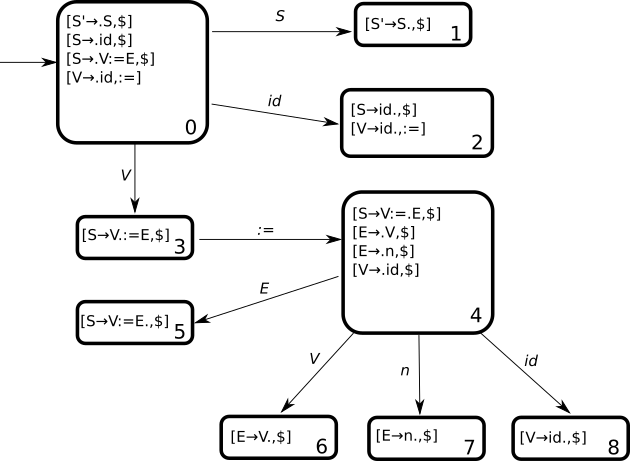
\includegraphics[width=\linewidth,height=\textheight,keepaspectratio]{figuras/iddfalr1.png}
\end{frame}

\begin{frame}
   \frametitle{Análise Sintática LALR(1)}
   \begin{itemize}
      \item O tamanho do DFA LR(1) se deve à existência de estados com o mesmos itens LR(0), mas com símbolos de verificação diferentes;
      \item a análise LALR(1) identifica tais estados e os combina;
      \item agora, o estado LALR(1) não tem um símbolo de verificação, mas sim um conjunto deles;
      \item \textbf{núcleo} de um estado LR(1): conjunto de itens LR(0) composto pelos primeiros componentes de todos os itens LR(1) no estado.
   \end{itemize}
\end{frame}

\begin{frame}
   \frametitle{Princípios da Análise Sintática LALR(1)}
   \begin{block}{Primeiro Princípio da Análise Sintática LALR(1)}
   O núcleo de um estado do DFA de itens LR(1) é um estado DFA de itens LR(0).
   \end{block}
 
   \begin{block}{Segundo Princípio da Análise Sintática LALR(1)}
   Dados dois estados $s_{1}$ e $s_{2}$ do DFA de itens LR(1) com o mesmo núcleo, suponha que exista uma transição em $X$ de $s_{1}$ para um estado $t_{1}$. Portanto, existe também uma transição em X do estado $s_{2}$ para o estado $t_{2}$, e os estados $t_{1}$ e $t_{2}$ têm o mesmo núcleo.
   \end{block}
   \textbf{DFA de itens LALR(1)}: a partir do autômato LR(1), identificar todos os estados com o mesmo núcleo e unir todos os símbolos de verificação correspondentes a um item LR(0) em um conjunto.
\end{frame}

\begin{frame}
   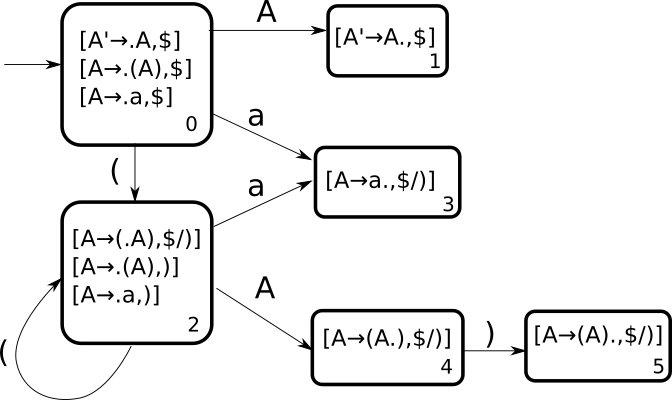
\includegraphics[width=\linewidth,height=\textheight,keepaspectratio]{figuras/aadfalalr1.png}
\end{frame}

\begin{frame}
   \frametitle{Consequências da Análise LALR(1)}
   \begin{itemize}
      \item O algoritmo para análise LALR(1) é o mesmo usado na LR(1);
      \item é possível que a transformação do autômato em LALR(1) cause conflitos inexistentes no autômato LR(1);
      \item na maioria das construções de linguagens de programação, esses conflitos não ocorrem;
      \item a \textbf{propagação de verificações à frente} permite computar o autômato LALR(1) diretamente a partir do autômato LR(0).
   \end{itemize}
\end{frame}

\section{YACC}
\begin{frame}[fragile]
   \frametitle{YACC - \textit{Yet Another Compiler Compiler}}
   \begin{block}{Gerador de Analisadores Sintáticos}
   Programa que recebe como entrada uma especificação da sintaxe de uma linguagem e produz como saída um procedimento de análise sintática para aquela linguagem. \\
   \$ sudo apt install bison
   \end{block}
   Arquivos \textbf{.y}:
   \begin{minted}{bash}
   {definições}
   %%
   {regras}
   %%
   {rotinas auxiliares}
   \end{minted}
\end{frame}

\begin{frame}
   \frametitle{Fundamentos do YACC}
   \begin{block}{Definições}
   Marcas, tipos de dados, regras gramaticais e diretivas \#include.
   \end{block}

   \begin{block}{Regras}
   Regras da gramática em BNF modificada, com $|$ para alternância, : no lugar de $\to$ e cada regra finalizada por ;.
   \end{block}
   
   \begin{block}{Rotinas Auxiliares}
   Declarações de procedimentos e unções que não estão em diretivas \#include.
   \end{block}
\end{frame}

\begin{frame}
   \frametitle{Gramática Exemplo para o YACC}
   $exp\to\textit{exp soma termo}|termo$ \\
   $soma\to+|-$ \\
   $termo\to\textit{termo mult fator}|fator$ \\
   $mult\to *$ \\
   $fator\to(exp)|\textbf{número}$
\end{frame}

\begin{frame}[fragile]
   \begin{minted}{c}
%{
#include <stdio.h>
#include <ctype.h>

int yylex(void);
int yyerror(char *);
%}

%token NUMBER
  \end{minted}
\end{frame}

\begin{frame}[fragile]
   \begin{minted}{c}
%%

command : exp { printf("%d\n", $1); }
        ; /* permite imprimir o resultado */

exp : exp '+' term { $$ = $1 + $3; }
    | exp '-' term { $$ = $1 + $3; }
    | term { $$ = $1; }
    ;
 
term : term '*' factor { $$ = $1 * $3; }
     | factor { $$ = $1 ;} 
     ;

factor : NUMBER { $$ = $1; }
       | '('exp')' { $$ = $2; }
       ;

   \end{minted}
\end{frame}

\begin{frame}[fragile]
   \scriptsize
   \begin{minted}{c}
%%

int main() {
   return yyparse();
}

int yylex(void) {
   int c;
   while ((c=getchar()) == ' '); /* elimina espaços em branco */
   if (isdigit(c)) {
      ungetc(c,stdin);
      scanf("%d", &yylval);
      return(NUMBER);
   }
   if (c == '\n') return 0; /* interrompe a análise sintática */
   return c;
}

/* imprimir a mensagem erro */
int yyerror(char *s) {
   fprintf(stderr, "%s\n", s);
   return 0;
}
   \end{minted}

\end{frame}


\section{Analisador Sintático para TINY em YACC}
\begin{frame}
   \frametitle{Analisador Sintático para TINY em YACC}
   \begin{itemize}
      \item No apêndice, há a listagem do código do analisador sintático para TINY em YACC;
      \item sua função \textit{yylex} invoca a função \textit{getToken} do analisador léxico do capítulo anterior sobre análise léxica;
      \item no lugar de operações aritméticas, ele utiliza as ações para construir a árvore abstrata;
      \item ao final, ele retorna a árvore formada para as próximas fases do compilador.
   \end{itemize}
\end{frame}

\section{Recuperação de Erros}
\begin{frame}
   \frametitle{Recuperação de Erros}
   \begin{itemize}
      \item Assim como no caso dos analisadores descendentes, não há técnica perfeita;
      \item novamente, uma abordagem \textbf{modo pânico};
      \item como existe um autômato, o analisado sabe por qual caminho retornar na presença de erros;
      \item o YACC permite ao desenvolvedor definir funções para o tratamento de erro de acordo com a gramática.
   \end{itemize}
\end{frame}

\begin{frame}
   \frametitle{Fim}
   Dúvidas?
\end{frame}

\end{document}
